\subsection{Vector Graphics}
Vector graphics is a form of computer graphics where mathematical expressions are used to describe an image. The image, or the 'scene', is made up of primitives that describe paths, lines and curves, and sometimes combinations of these in order to create more complex shapes.

By relying on mathematical expressions instead of pixel values relative to screen resolution, vector graphics can be described as resolution independent. This is often conceptualized in the form of scaling: While scaling a rasterized image will result in a blurry image, scaling a vectorized image will result in the mathematical expressions being recalculated, and the image will remain sharp. This process is visualized in figure \ref{fig:vectorscaling}

\begin{figure}[h!]
\centering 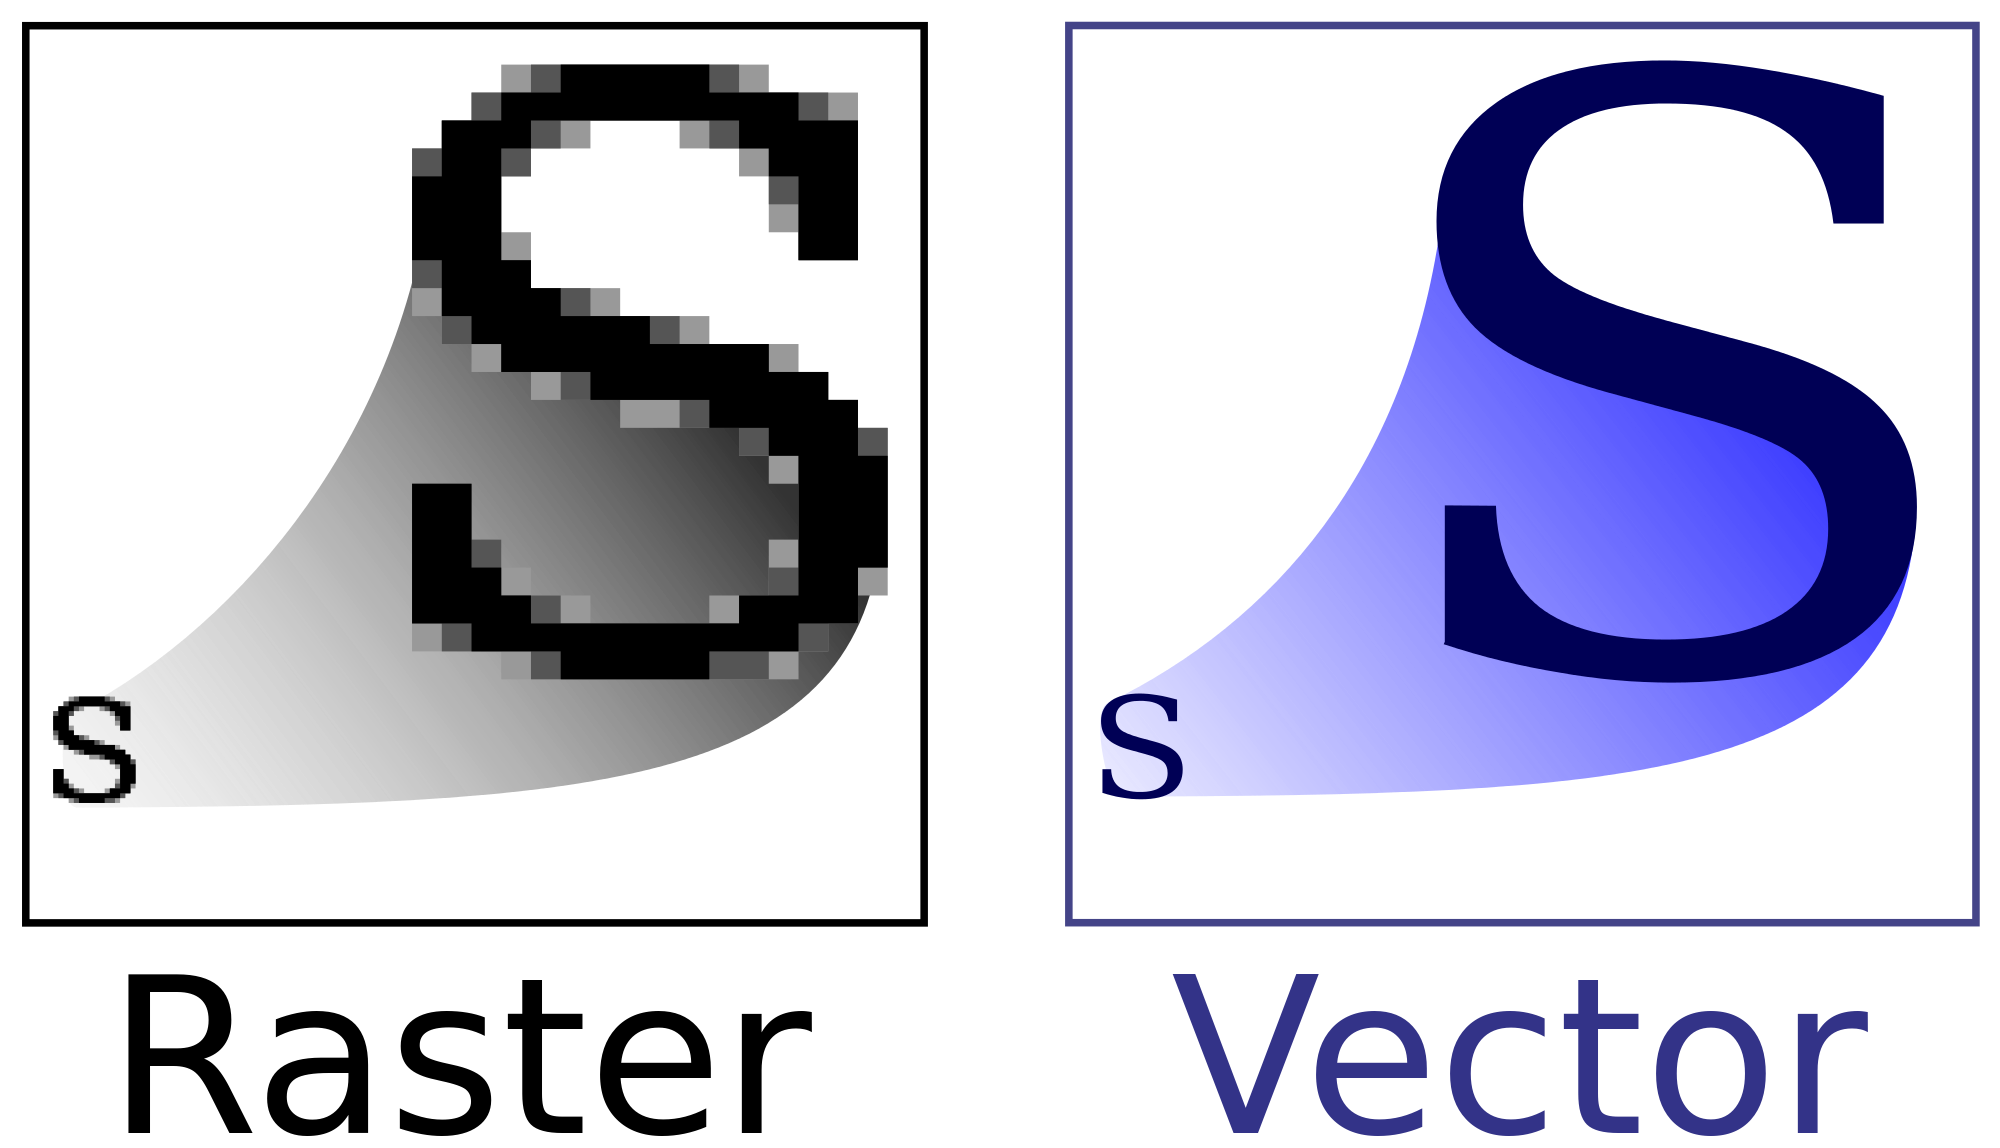
\includegraphics[width=0.5\linewidth]{images/bm_vs_svg.png}
\caption{Scaling comparison between raster graphics (left) and vector grahics (right). Source: \cite{svg}}
\label{fig:vectorscaling}
\end{figure}

Vector graphics are predominantly used to describe 2D graphics, in order to distinguish them from 2D raster graphics, which is described later on. In 3D graphics, most implementations utilize points, lines and curves to define shapes, which makes them a lot like vector graphics. Voxel graphics is an implementation of 3D graphics that tries to define it's shapes by utilizing three dimensional pixels, so-called 'voxels', but is rarely used.

Some computer font types, like TrueType uses vector graphics and more specifically Bézier curves to represent glyphs\cite{truetype}. // Is this necessary?

Due to the geometrical nature of vectors, it's not practical to use vector graphics to represent photographs. Computer generated text, drawings or imagery, for use in graphical design, is the most common use case for vector graphics today, since the graphic can easily be scaled up or down by demand. Most professional image processing and design software, e.g. Adobe Illustrator, support vector graphics. To store the graphics, file formats such as \texttt{.ai} (for use in Adobe Illustrator) or the open standard \texttt{.svg} (Scalable Vector Graphics) can be used.
